% Session 19 – LSTM: Short vs Long-Term Dependency and Gates
% Deep Learning Course, IIITDwd
% Instructors: Prof. S R M Prasanna & Dr. Sunil Saumya

\documentclass[12pt,a4paper]{article}
\usepackage{amsmath,amsthm,amssymb,mathtools}
\usepackage{tikz}
\usetikzlibrary{arrows.meta,positioning,shapes.geometric,calc,fit,backgrounds}
\usepackage{graphicx}
\usepackage{booktabs,tabularx,multirow}
\usepackage[ruled,vlined,linesnumbered]{algorithm2e}
\usepackage[most]{tcolorbox}
\usepackage{hyperref}
\usepackage[capitalize,noabbrev]{cleveref}
\usepackage[margin=1in]{geometry}
\usepackage{fancyhdr}
\usepackage{enumitem}
\usepackage{xcolor}

%% ── tcolorbox environments ──────────────────────────────────────────────────
\newtcolorbox{keyinsight}[1][]{colback=blue!5!white,colframe=blue!75!black,
  fonttitle=\bfseries,title=Key Insight,#1}
\newtcolorbox{example}[1][]{colback=green!5!white,colframe=green!75!black,
  fonttitle=\bfseries,title=Example,#1}
\newtcolorbox{warningbox}[1][]{colback=red!5!white,colframe=red!75!black,
  fonttitle=\bfseries,title=Warning,#1}

%% ── amsthm environments ─────────────────────────────────────────────────────
\newtheorem{theorem}{Theorem}[section]
\newtheorem{lemma}[theorem]{Lemma}
\newtheorem{definition}{Definition}[section]
\newtheorem{remark}{Remark}[section]

%% ── Page style ───────────────────────────────────────────────────────────────
\pagestyle{fancy}
\fancyhf{}
\rhead{Deep Learning -- Session 19}
\lhead{LSTM: Short vs Long-Term Dependency}
\cfoot{\thepage}
\renewcommand{\headrulewidth}{0.4pt}

%% ── Hyperref ─────────────────────────────────────────────────────────────────
\hypersetup{
  colorlinks=true,
  linkcolor=blue!60!black,
  citecolor=green!50!black,
  urlcolor=blue!70!black,
  pdftitle={Session 19 -- LSTM: Short vs Long-Term Dependency and Gates},
  pdfauthor={IIITDwd Deep Learning Course}
}

% ─────────────────────────────────────────────────────────────────────────────
\begin{document}

%% ── Title page ───────────────────────────────────────────────────────────────
\begin{titlepage}
  \centering
  \vspace*{2cm}
  {\LARGE\bfseries Deep Learning Course\\[0.4em]
   Indian Institute of Information Technology Dharwad\\[1.5em]}
  \rule{\linewidth}{1pt}\\[0.8em]
  {\huge\bfseries Session 19\\[0.5em]
   Long Short-Term Memory (LSTM):\\[0.3em]
   Short vs Long-Term Dependency and Gates}\\[0.8em]
  \rule{\linewidth}{1pt}\\[1.5em]
  \begin{tabular}{ll}
    \textbf{Session Number:} & 19 \\[0.4em]
    \textbf{Topic:}          & LSTM motivation, vanishing gradient, gate mechanism \\[0.4em]
    \textbf{Date:}           & January 24, 2026 \\[0.4em]
    \textbf{Duration:}       & $\approx 1$h\,39m \\[0.4em]
    \textbf{Instructors:}    & Prof.\ S.\ R.\ Mahadeva Prasanna \\
                             & Dr.\ Sunil Saumya \\[0.4em]
    \textbf{Slide Decks:}    & \texttt{05-DL-RNN} (slides 30, 35, 37/63) \\
                             & \texttt{06-RNNTypesBackpropagation} (slide 20/22) \\
  \end{tabular}
  \vfill
  {\large\itshape Acknowledgement: Colah's Blog --
   ``Understanding LSTM Networks''}\\[1em]
  {\large IIITDwd -- B.Tech Deep Learning, 2025--26}
\end{titlepage}

%% ── Table of contents ────────────────────────────────────────────────────────
\tableofcontents
\newpage

% =============================================================================
\section{Introduction}
\label{sec:introduction}
% =============================================================================

Session~19 of the IIITDwd Deep Learning course marks the transition from
standard Recurrent Neural Networks (RNNs) to the Long Short-Term Memory
(LSTM) architecture. The session was delivered jointly by
Prof.\ S.\ R.\ Mahadeva Prasanna and Dr.\ Sunil Saumya and draws primarily
from two slide decks: \texttt{05-DL-RNN} and
\texttt{06-RNNTypesBackpropagation}.

The central thesis of the session is that standard RNNs, while capable of
modelling \emph{short-term} sequential dependencies, fundamentally fail on
\emph{long-term} dependencies because gradients vanish as they propagate
backwards through many time steps. The LSTM architecture, proposed by
Hochreiter and Schmidhuber (1997), addresses this failure through two
complementary innovations:

\begin{enumerate}[label=\textbf{\arabic*.}]
  \item A dedicated \textbf{cell-state highway} $C_t$ that carries long-term
        context with only minor, additive interactions --- preventing the
        multiplicative gradient decay that cripples plain RNNs.
  \item A set of three \textbf{gates} (forget, input, output), each
        implemented as a sigmoid neural network, that selectively read,
        write, and erase information on the cell-state line.
\end{enumerate}

\begin{keyinsight}[title=Session Objective]
By the end of Session~19 students should be able to: (i) articulate why
plain RNNs fail on long-range context using the gradient-vanishing argument;
(ii) describe the two-line (cell-state + hidden-state) feedback structure of
LSTM; and (iii) explain the role of each of the three gates at a conceptual
level. Numerical gate computations are deferred to Session~20.
\end{keyinsight}

% =============================================================================
\section{Background and Prerequisites}
\label{sec:background}
% =============================================================================

\subsection{Sequence Modelling and the RNN Recap}
\label{subsec:rnn-recap}

Before LSTM can be appreciated, it is essential to recall the operation of a
vanilla RNN cell. At each time step $t$ the hidden state is updated as

\begin{equation}
  \label{eq:rnn-update}
  h_t = \tanh\!\bigl(W_{hh}\,h_{t-1} + W_{xh}\,x_t + b_h\bigr),
\end{equation}

where $x_t \in \mathbb{R}^{d}$ is the input vector, $h_{t-1} \in
\mathbb{R}^{n}$ is the previous hidden state, $W_{hh} \in \mathbb{R}^{n
\times n}$ and $W_{xh} \in \mathbb{R}^{n \times d}$ are learnable weight
matrices, and $b_h$ is a bias vector. The output at each time step (e.g.\
for language modelling) is

\begin{equation}
  \label{eq:rnn-output}
  \hat{y}_t = \text{softmax}(W_{hy}\,h_t + b_y).
\end{equation}

The feedback loop through $h_{t-1}$ gives the RNN its \emph{memory}: at
time step $t$ the hidden state encodes a compressed representation of all
tokens seen so far. As the instructors emphasised,

\begin{quote}
``The goal [in language modelling] is, given one word or a set of words in a
given sequence, predict the next word.'' \hfill (Dr.\ Sunil Saumya, 00:15)
\end{quote}

\subsection{What Is Short-Term Dependency?}
\label{subsec:short-term}

\begin{definition}[Short-Term Dependency]
  \label{def:short-term}
  A prediction task exhibits \emph{short-term dependency} when the
  relevant context lies within a small, fixed window immediately preceding
  the prediction point. A standard RNN with a shallow hidden state suffices
  for such tasks.
\end{definition}

\begin{example}[title=``The clouds are in the \underline{\hspace{1.5em}}'']
  Given the phrase ``the clouds are in the'', any fluent speaker immediately
  predicts ``sky''. The information required (clouds, in, the) is entirely
  local --- the gap between evidence and prediction is negligible. This is a
  classic short-term dependency, and a vanilla RNN handles it well.
\end{example}

\subsection{What Is Long-Term Dependency?}
\label{subsec:long-term}

\begin{definition}[Long-Term Dependency]
  \label{def:long-term}
  A prediction task exhibits \emph{long-term dependency} when the evidence
  needed to make a correct prediction lies many time steps before the
  prediction point, so that the gap between relevant context and usage is
  large.
\end{definition}

The canonical classroom example from the slide deck (V01, 00:18:55) is
reproduced below.

\begin{example}[title=Karnataka/Delhi/Hindi Example (V01)]
  \textit{``I am from a South Indian family, specifically Karnataka, but
  settled in Delhi. I had spent most of my childhood and done schooling as
  well as college education in Delhi. Apart from Kannada, I can speak
  fluent \underline{\hspace{1.5em}} also.''}

  \medskip
  \noindent The missing word is ``Hindi''. The \emph{short-term} context
  (``Apart from Kannada, I can speak fluent'') tells us to expect a
  \emph{language name} but is ambiguous about \emph{which} language.
  To resolve the ambiguity we need the long-range context
  ``settled in Delhi'' --- many tokens earlier. A standard RNN with
  vanishing gradients cannot bridge this gap.
\end{example}

% =============================================================================
\section{Why Standard RNNs Fail on Long-Range Context}
\label{sec:rnn-failure}
% =============================================================================

\subsection{Backpropagation Through Time (BPTT)}
\label{subsec:bptt}

Training RNNs uses Backpropagation Through Time (BPTT), which unrolls the
network across all $T$ time steps and applies the chain rule. The gradient
of the loss $\mathcal{L}$ with respect to the hidden state at an early time
step $t$ passes through every intermediate step:

\begin{align}
  \label{eq:bptt-chain}
  \frac{\partial \mathcal{L}}{\partial h_t}
  &= \frac{\partial \mathcal{L}}{\partial h_T}
     \prod_{k=t+1}^{T}
     \frac{\partial h_k}{\partial h_{k-1}}.
\end{align}

Each factor in the product is

\begin{equation}
  \label{eq:jacobian-factor}
  \frac{\partial h_k}{\partial h_{k-1}}
  = W_{hh}^{\top} \operatorname{diag}\!\bigl(\tanh'(a_{k-1})\bigr),
\end{equation}

where $a_{k-1} = W_{hh}h_{k-2} + W_{xh}x_{k-1} + b_h$ is the
pre-activation. Since $|\tanh'(z)| \leq 1$ for all $z$, the spectral norm
of each factor is bounded by $\|W_{hh}\|_2$.

\subsection{The Vanishing Gradient Problem}
\label{subsec:vanishing}

\begin{theorem}[Gradient Magnitude Decay]
  \label{thm:vanishing}
  Let $\gamma = \|W_{hh}\|_2 \cdot \max_z|\tanh'(z)|$. If $\gamma < 1$,
  then
  \begin{equation}
    \label{eq:vanishing-bound}
    \left\|\frac{\partial \mathcal{L}}{\partial h_t}\right\|
    \;\leq\;
    \left\|\frac{\partial \mathcal{L}}{\partial h_T}\right\|
    \cdot \gamma^{T-t}.
  \end{equation}
  The gradient at step $t$ decays \emph{exponentially} with the distance
  $T - t$ from the output.
\end{theorem}

\begin{example}[title=Numerical Illustration (V04 scenario)]
  Consider the sentence ``I am from France \ldots\ I speak fluent
  \underline{\hspace{1em}}'' (slide 20/22 of \texttt{06-RNNTypesBackpropagation}).
  Suppose the sequence has $T = 6$ steps and $\gamma \approx 0.5$. The
  gradient arriving at the first token (``France'') is
  \[
    \|\nabla_{h_1}\| \;\leq\; \|\nabla_{h_6}\| \cdot (0.5)^{5}
    \;=\; \|\nabla_{h_6}\| \cdot 0.03125.
  \]
  That is, only $\approx 3\%$ of the gradient signal from the output
  reaches the earliest relevant token --- effectively zero for learning.
\end{example}

\cref{fig:rnn-fail} illustrates the gradient flow for this scenario.

\begin{figure}[ht]
  \centering
  % ── TikZ: RNN Long-Dependency Failure ─────────────────────────────────────
  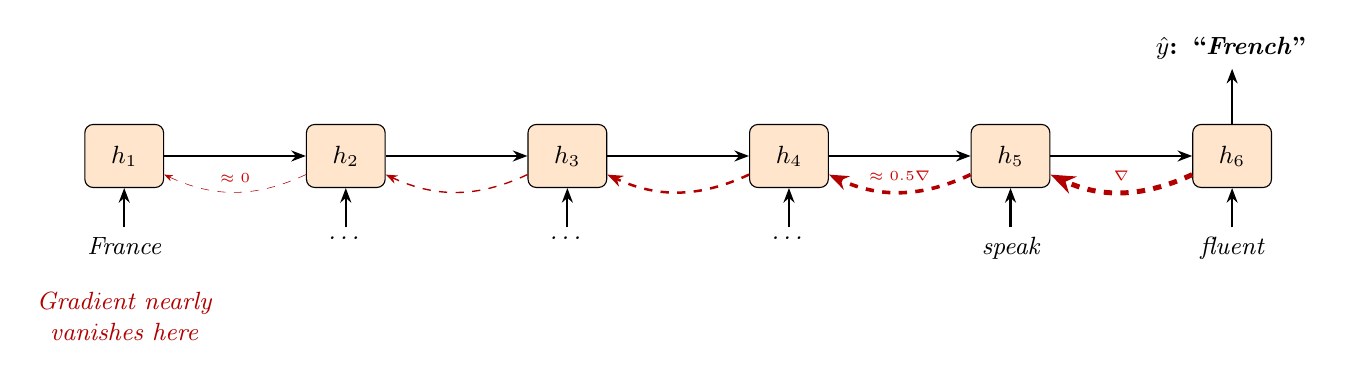
\begin{tikzpicture}[
      node distance=1.4cm and 1.8cm,
      cell/.style={draw,rounded corners=3pt,minimum width=1.0cm,
                   minimum height=0.8cm,fill=orange!20,font=\small},
      word/.style={font=\small\itshape},
      arr/.style={-{Stealth[scale=0.8]},thick},
      garr/.style={-{Stealth[scale=0.8]},thick,red!70!black,dashed},
    ]
    \node[cell] (h1) {$h_1$};
    \node[cell,right=of h1] (h2) {$h_2$};
    \node[cell,right=of h2] (h3) {$h_3$};
    \node[cell,right=of h3] (h4) {$h_4$};
    \node[cell,right=of h4] (h5) {$h_5$};
    \node[cell,right=of h5] (h6) {$h_6$};

    % forward arrows
    \draw[arr] (h1)--(h2);
    \draw[arr] (h2)--(h3);
    \draw[arr] (h3)--(h4);
    \draw[arr] (h4)--(h5);
    \draw[arr] (h5)--(h6);

    % input words
    \node[word,below=0.5cm of h1] (w1) {France};
    \node[word,below=0.5cm of h2] (w2) {\ldots};
    \node[word,below=0.5cm of h3] (w3) {\ldots};
    \node[word,below=0.5cm of h4] (w4) {\ldots};
    \node[word,below=0.5cm of h5] (w5) {speak};
    \node[word,below=0.5cm of h6] (w6) {fluent};

    \draw[arr] (w1)--(h1);
    \draw[arr] (w2)--(h2);
    \draw[arr] (w3)--(h3);
    \draw[arr] (w4)--(h4);
    \draw[arr] (w5)--(h5);
    \draw[arr] (w6)--(h6);

    % output
    \node[above=0.7cm of h6,font=\small\bfseries] (yhat) {$\hat{y}$: ``\textit{French}''};
    \draw[arr] (h6)--(yhat);

    % backward gradient arrows (dashed red, fading)
    \draw[garr,line width=1.8pt] (h6) to[bend left=25]
          node[above,font=\tiny,red!80!black]{$\nabla$} (h5);
    \draw[garr,line width=1.3pt] (h5) to[bend left=25]
          node[above,font=\tiny,red!80!black]{$\approx 0.5\nabla$} (h4);
    \draw[garr,line width=0.9pt] (h4) to[bend left=25] (h3);
    \draw[garr,line width=0.5pt] (h3) to[bend left=25] (h2);
    \draw[garr,line width=0.2pt] (h2) to[bend left=25]
          node[above,font=\tiny,red!80!black]{$\approx 0$} (h1);

    % annotation
    \node[below=1.2cm of h1,text=red!70!black,font=\small\itshape,
          align=center] {Gradient nearly\\vanishes here};
  \end{tikzpicture}
  \caption{Gradient flow in a plain RNN processing a long-dependency
           sentence. The dashed red arrows show the gradient magnitude
           decaying from right (output) to left (early token ``France'').
           By the time the gradient reaches $h_1$, it is negligibly small,
           so the network cannot learn that ``France'' determines the
           answer.}
  \label{fig:rnn-fail}
\end{figure}

\subsection{Exploding Gradients}
\label{subsec:exploding}

The complementary failure mode occurs when $\gamma > 1$: the gradient grows
\emph{exponentially}, causing numerical overflow and training instability.
As \cref{eq:vanishing-bound} shows, the regime $\gamma < 1$ causes
vanishing and $\gamma > 1$ causes explosion --- both are pathological.

\begin{warningbox}[title=Vanishing vs Exploding Gradient]
  The plain RNN \cref{eq:rnn-update} is unstable in the BPTT sense:
  \begin{itemize}[nosep]
    \item If $\|W_{hh}\|_2 \cdot \max|\tanh'| < 1$: gradients
          \textbf{vanish} --- long-term dependencies cannot be learned.
    \item If $\|W_{hh}\|_2 \cdot \max|\tanh'| > 1$: gradients
          \textbf{explode} --- training diverges.
  \end{itemize}
  Gradient clipping (heuristic) can partially address explosion, but
  vanishing requires an architectural fix --- which is precisely what
  LSTM provides.
\end{warningbox}

\subsection{Short-Term vs Long-Term: A Practical Comparison}
\label{subsec:comparison}

\cref{tab:rnn-lstm-comparison} summarises the empirical performance
difference observed by the instructors (confirmed via a TA experiment on
sentiment classification):

\begin{table}[ht]
  \centering
  \caption{RNN vs LSTM accuracy (\%) on sentiment classification for
           varying sequence lengths. Longer sequences magnify the RNN
           performance gap (illustrative values from lecture).}
  \label{tab:rnn-lstm-comparison}
  \begin{tabular}{@{}lcc@{}}
    \toprule
    \textbf{Sequence Length} & \textbf{Plain RNN (\%)} & \textbf{LSTM (\%)} \\
    \midrule
    50  & 81.0 & 81.6 \\
    100 & 81.6 & 82.0 \\
    200 & $\downarrow$ (degraded) & 85.0 \\
    \midrule
    \multicolumn{3}{@{}l@{}}{\small As sequence length increases, RNN
    accuracy degrades gracefully then plateaus at a lower value.} \\
    \bottomrule
  \end{tabular}
\end{table}

\begin{keyinsight}[title=Task-Dependent Architecture Choice]
  It is \emph{not} always the case that LSTM outperforms RNN. For
  purely short-term tasks, LSTM adds computational overhead (roughly
  $4\times$ more parameters per cell) with negligible accuracy gain.
  LSTM is warranted when the task genuinely requires long-range context.
\end{keyinsight}

% =============================================================================
\section{The LSTM Architecture: Motivation and Design}
\label{sec:lstm-design}
% =============================================================================

\subsection{Design Rationale: Two Feedback Lines}
\label{subsec:two-lines}

The instructors motivated the LSTM design from first principles. The
insight is that a plain RNN has \emph{one} feedback line (the hidden state
$h_{t-1}$) which conflates short-term and long-term context:

\begin{quote}
``The first [idea] was we need two feedback parts. One, to keep track of the
short-term context information. Another to keep track of the long-term
context information.'' \hfill (Prof.\ Prasanna, 00:25)
\end{quote}

This motivates the dual-state design:

\begin{itemize}
  \item \textbf{Hidden state} $h_t$: the lower feedback line; carries
        short-term sequence knowledge (identical in spirit to a plain RNN
        hidden state).
  \item \textbf{Cell state} $C_t$: the upper feedback line; a
        \emph{memory highway} that preserves long-term context across
        potentially many time steps.
\end{itemize}

Between these two lines, \textbf{gate mechanisms} regulate the flow of
information: deciding what to write to $C_t$, what to erase from $C_t$,
and how much of $C_t$ to expose in $h_t$.

\subsection{The Cell State Highway}
\label{subsec:cell-state}

The cell state $C_t$ is the defining innovation. As Prof.\ Prasanna
explained:

\begin{quote}
``The cell state is the horizontal line running through the top of the
diagram. LSTM can remove or add information to the cell state, regulated by
structures called gates.''
\end{quote}

The key property is that updates to $C_t$ are \emph{additive}, not
multiplicative:

\begin{equation}
  \label{eq:cell-state-update}
  C_t = f_t \odot C_{t-1} + i_t \odot \tilde{C}_t,
\end{equation}

where $\odot$ denotes element-wise (Hadamard) multiplication, $f_t$ is
the forget-gate vector, $i_t$ is the input-gate vector, and $\tilde{C}_t$
is the candidate cell state. The gradient of $C_t$ with respect to
$C_{t-1}$ is simply $f_t$ --- a diagonal matrix with entries in $[0,1]$.
There is no repeated multiplication by $W_{hh}$ or $\tanh'$ along this
path, so gradients can flow unobstructed over long distances.

\begin{keyinsight}[title=Additive Updates Prevent Vanishing Gradients]
  In a plain RNN the gradient through time is a \emph{product} of Jacobians
  (\cref{eq:bptt-chain}), causing exponential decay. On the LSTM cell-state
  highway the gradient path reduces to a \emph{sum} modulated only by the
  forget gate. This is the fundamental mechanism by which LSTM overcomes the
  vanishing gradient problem.
\end{keyinsight}

% =============================================================================
\section{Gates in LSTM}
\label{sec:gates}
% =============================================================================

\subsection{The Gate Concept}
\label{subsec:gate-concept}

A \textbf{gate} in LSTM is a combination of a sigmoid neural network and a
pointwise multiplication (slide 37/63 of \texttt{05-DL-RNN}, V02 at
00:38:50):

\begin{equation}
  \label{eq:gate-generic}
  g_t = \sigma\!\bigl(W_g\,[h_{t-1},\,x_t] + b_g\bigr),
\end{equation}

where $\sigma(\cdot)$ is the sigmoid function, $[h_{t-1}, x_t]$ denotes
the concatenation of the previous hidden state and the current input, and
$W_g$, $b_g$ are learnable parameters specific to gate $g$. The output
$g_t \in [0,1]^n$ is then applied element-wise to the vector being gated:

\begin{equation}
  \label{eq:gate-apply}
  \text{gated output} = g_t \odot \text{input vector}.
\end{equation}

\begin{keyinsight}[title=Sigmoid as a Soft Gate]
  Unlike a digital logic gate (binary 0 or 1), an LSTM gate produces
  \emph{continuous} values in $[0,1]$ per dimension. A value of 0 means
  ``block this dimension completely''; a value of 1 means ``pass this
  dimension through unchanged''; intermediate values scale the
  information proportionally. This differentiability is what allows
  backpropagation to train the gate parameters.
\end{keyinsight}

\cref{fig:gate-diagram} shows the structure of a single LSTM gate.

\begin{figure}[ht]
  \centering
  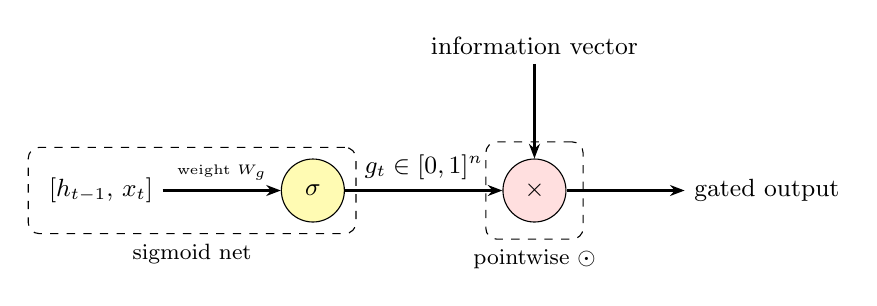
\begin{tikzpicture}[
      node distance=1.2cm,
      sig/.style={draw,circle,minimum size=0.8cm,fill=yellow!30,font=\small},
      mul/.style={draw,circle,minimum size=0.8cm,fill=pink!50,font=\small},
      arr/.style={-{Stealth[scale=0.8]},thick},
      lbl/.style={font=\small},
    ]
    % input
    \node[lbl] (inp) {$[h_{t-1},\,x_t]$};
    % sigmoid block
    \node[sig,right=1.5cm of inp] (sig) {$\sigma$};
    % multiply
    \node[mul,right=2.0cm of sig] (mult) {$\times$};
    % info stream from above
    \node[lbl,above=1.2cm of mult] (stream) {information vector};
    % output
    \node[lbl,right=1.5cm of mult] (out) {gated output};

    \draw[arr] (inp)--(sig) node[midway,above,font=\tiny]{weight $W_g$};
    \draw[arr] (sig)--(mult) node[midway,above,font=\small]{$g_t \in [0,1]^n$};
    \draw[arr] (stream)--(mult);
    \draw[arr] (mult)--(out);

    % annotation boxes
    \node[draw,dashed,rounded corners,
          fit=(inp)(sig),inner sep=4pt,
          label=below:{\footnotesize sigmoid net}] {};
    \node[draw,dashed,rounded corners,
          fit=(mult),inner sep=6pt,
          label=below:{\footnotesize pointwise $\odot$}] {};
  \end{tikzpicture}
  \caption{Structure of a single LSTM gate (slide 37/63, V02). The sigmoid
           layer maps the concatenated input to a gating vector $g_t \in
           [0,1]^n$, which is then multiplied element-wise with the
           information vector to selectively allow or block information.}
  \label{fig:gate-diagram}
\end{figure}

\subsection{The Three Gates of LSTM}
\label{subsec:three-gates}

LSTM uses three gates, each with independent weight matrices, to regulate
the cell state $C_t$:

\subsubsection{Forget Gate $f_t$}
\label{subsubsec:forget}

The forget gate decides how much of the \emph{previous} cell state $C_{t-1}$
to retain:

\begin{equation}
  \label{eq:forget-gate}
  f_t = \sigma\!\bigl(W_f\,[h_{t-1},\,x_t] + b_f\bigr).
\end{equation}

When $f_t \approx \mathbf{0}$, the previous cell state is completely
erased (``forgotten''). When $f_t \approx \mathbf{1}$, it is fully
preserved. As the instructor stated:

\begin{quote}
``One means completely keep this dimension, zero means completely get rid of
this dimension. So that is the purpose of forgetting it.''
\hfill (Prof.\ Prasanna, 00:41)
\end{quote}

\subsubsection{Input Gate $i_t$ and Candidate Cell State $\tilde{C}_t$}
\label{subsubsec:input}

The input gate decides which components of the \emph{current} information
should be written to the cell state:

\begin{align}
  \label{eq:input-gate}
  i_t &= \sigma\!\bigl(W_i\,[h_{t-1},\,x_t] + b_i\bigr), \\
  \label{eq:candidate}
  \tilde{C}_t &= \tanh\!\bigl(W_C\,[h_{t-1},\,x_t] + b_C\bigr).
\end{align}

The candidate $\tilde{C}_t \in [-1,1]^n$ is the new information proposed
by the standard RNN operation ($\tanh$ of the weighted input). The gate
$i_t$ decides how much of this candidate actually enters the cell state.

\begin{remark}
  \label{rem:input-gate-naming}
  The instructors noted a common naming confusion: in Gated Recurrent
  Units (GRU) the analogous gate is called the \emph{update gate}, whereas
  in LSTM it is called the \emph{input gate}. Both serve the same
  conceptual purpose of writing new information into the memory.
\end{remark}

\subsubsection{Cell State Update}
\label{subsubsec:cell-update}

The cell state is updated by combining the forget and input gate outputs:

\begin{equation}
  \label{eq:cell-update}
  C_t = f_t \odot C_{t-1} + i_t \odot \tilde{C}_t.
\end{equation}

The additive structure of \cref{eq:cell-update} is what makes $C_t$ a
gradient highway: $\partial C_t / \partial C_{t-1} = f_t$, which is not
repeatedly multiplied across time steps.

\subsubsection{Output Gate $o_t$}
\label{subsubsec:output}

The output gate determines how much of the cell state to expose as the
hidden state $h_t$:

\begin{align}
  \label{eq:output-gate}
  o_t &= \sigma\!\bigl(W_o\,[h_{t-1},\,x_t] + b_o\bigr), \\
  \label{eq:hidden-update}
  h_t &= o_t \odot \tanh(C_t).
\end{align}

The $\tanh$ squashes $C_t$ into $[-1,1]$ before the gate is applied,
keeping the hidden state bounded.

\subsection{Summary of LSTM Equations}
\label{subsec:lstm-equations}

The complete set of LSTM equations for one time step is:

\begin{align}
  f_t          &= \sigma(W_f\,[h_{t-1},x_t] + b_f)
                 \label{eq:lstm-f} \\
  i_t          &= \sigma(W_i\,[h_{t-1},x_t] + b_i)
                 \label{eq:lstm-i} \\
  \tilde{C}_t  &= \tanh(W_C\,[h_{t-1},x_t] + b_C)
                 \label{eq:lstm-Ctil} \\
  C_t          &= f_t \odot C_{t-1} + i_t \odot \tilde{C}_t
                 \label{eq:lstm-C} \\
  o_t          &= \sigma(W_o\,[h_{t-1},x_t] + b_o)
                 \label{eq:lstm-o} \\
  h_t          &= o_t \odot \tanh(C_t)
                 \label{eq:lstm-h}
\end{align}

\cref{tab:lstm-params} catalogues the learnable parameter matrices.

\begin{table}[ht]
  \centering
  \caption{Learnable parameters in a single LSTM cell with hidden size $n$
           and input size $d$. Each gate has its own weight matrix and bias.}
  \label{tab:lstm-params}
  \begin{tabular}{@{}llll@{}}
    \toprule
    \textbf{Gate / State} & \textbf{Weight Matrix} & \textbf{Shape} & \textbf{Bias Shape} \\
    \midrule
    Forget gate $f_t$      & $W_f$ & $n \times (n+d)$ & $n$ \\
    Input gate $i_t$       & $W_i$ & $n \times (n+d)$ & $n$ \\
    Candidate $\tilde{C}_t$ & $W_C$ & $n \times (n+d)$ & $n$ \\
    Output gate $o_t$      & $W_o$ & $n \times (n+d)$ & $n$ \\
    \midrule
    \multicolumn{4}{@{}l@{}}{\small Total parameters: $4n(n+d) + 4n = 4n(n+d+1)$} \\
    \bottomrule
  \end{tabular}
\end{table}

% =============================================================================
\section{LSTM Cell Architecture: Diagram and Walk-Through}
\label{sec:lstm-cell}
% =============================================================================

\subsection{The Full LSTM Cell Diagram}
\label{subsec:lstm-cell-diagram}

\cref{fig:lstm-cell} shows the full LSTM recurrence cell in the style of
Colah's blog (referenced in slides 35/63 of \texttt{05-DL-RNN}, V03 and V05).

\begin{figure}[ht]
  \centering
  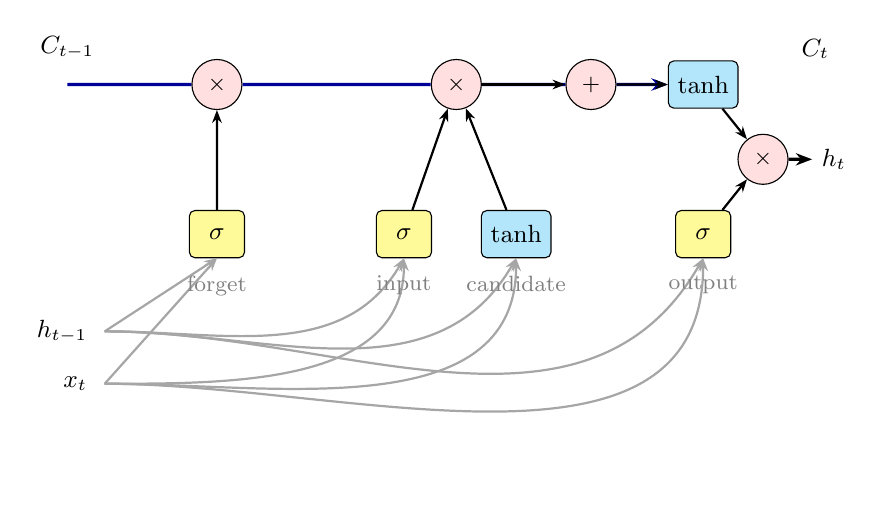
\begin{tikzpicture}[
      scale=0.95,
      node distance=0.9cm and 1.1cm,
      sig/.style={draw,rounded corners=2pt,minimum width=0.7cm,
                  minimum height=0.6cm,fill=yellow!40,font=\small},
      tnh/.style={draw,rounded corners=2pt,minimum width=0.7cm,
                  minimum height=0.6cm,fill=cyan!30,font=\small},
      op/.style={draw,circle,minimum size=0.55cm,fill=pink!50,font=\footnotesize},
      arr/.style={-{Stealth[scale=0.7]},thick},
      lbl/.style={font=\small},
    ]

    % ── Cell state (top horizontal line) ──────────────────────────────────
    \coordinate (CL) at (0,3.5);
    \coordinate (CR) at (10,3.5);

    % ── Forget gate ────────────────────────────────────────────────────────
    \node[sig]  (fg)  at (2.0,1.5) {$\sigma$};
    \node[op]   (fmul) at (2.0,3.5) {$\times$};

    % ── Input gate + candidate ─────────────────────────────────────────────
    \node[sig]  (ig)  at (4.5,1.5) {$\sigma$};
    \node[tnh]  (cand) at (6.0,1.5) {$\tanh$};
    \node[op]   (imul) at (5.2,3.5) {$\times$};
    \node[op]   (iadd) at (7.0,3.5) {$+$};

    % ── Output gate ────────────────────────────────────────────────────────
    \node[sig]  (og)  at (8.5,1.5) {$\sigma$};
    \node[tnh]  (otanh) at (8.5,3.5) {$\tanh$};
    \node[op]   (omul) at (9.3,2.5) {$\times$};

    % ── Cell state line ────────────────────────────────────────────────────
    \draw[arr,line width=1.2pt,blue!60!black]
          (CL) -- (fmul) -- (imul) -- (iadd) -- (otanh);

    % ── Forget gate connections ────────────────────────────────────────────
    \draw[arr] (fg) -- (fmul);

    % ── Input gate connections ─────────────────────────────────────────────
    \draw[arr] (ig)   -- (imul);
    \draw[arr] (cand) -- (imul);
    \draw[arr] (imul) -- (iadd);

    % ── Output gate connections ────────────────────────────────────────────
    \draw[arr] (iadd) -- (otanh);
    \draw[arr] (otanh) -- (omul);
    \draw[arr] (og)  -- (omul);

    % ── Input h_{t-1} and x_t (shared concatenated input) ─────────────────
    \coordinate (htminus1) at (0.5, 0.2);
    \node[lbl,left=0.1cm of htminus1] {$h_{t-1}$};
    \coordinate (xt)       at (0.5, -0.5);
    \node[lbl,left=0.1cm of xt] {$x_t$};

    % feed all gates
    \draw[arr,gray!70] (htminus1) -- (fg.south);
    \draw[arr,gray!70] (xt)       -- (fg.south);
    \draw[arr,gray!70] (htminus1) to[out=0,in=240] (ig.south);
    \draw[arr,gray!70] (xt)       to[out=0,in=270] (ig.south);
    \draw[arr,gray!70] (htminus1) to[out=0,in=240] (cand.south);
    \draw[arr,gray!70] (xt)       to[out=0,in=270] (cand.south);
    \draw[arr,gray!70] (htminus1) to[out=0,in=240] (og.south);
    \draw[arr,gray!70] (xt)       to[out=0,in=270] (og.south);

    % ── Outputs ────────────────────────────────────────────────────────────
    \node[lbl,right=0.3cm of omul] (ht) {$h_t$};
    \draw[arr,line width=1.2pt] (omul) -- (ht);

    \node[lbl,above=0.2cm of CR] {$C_t$};
    \node[lbl,above=0.2cm of CL] {$C_{t-1}$};

    % ── Labels ─────────────────────────────────────────────────────────────
    \node[below=0.1cm of fg,  font=\footnotesize,text=gray] {forget};
    \node[below=0.1cm of ig,  font=\footnotesize,text=gray] {input};
    \node[below=0.1cm of cand,font=\footnotesize,text=gray] {candidate};
    \node[below=0.1cm of og,  font=\footnotesize,text=gray] {output};

  \end{tikzpicture}
  \caption{LSTM recurrence cell (after Colah's blog, referenced in slides
           35/63 of \texttt{05-DL-RNN}, V03). The thick blue horizontal line
           is the \textbf{cell state} $C_t$ --- the long-term memory highway.
           Yellow $\sigma$ blocks are sigmoid gates; cyan $\tanh$ blocks
           produce bounded values. Pink circles denote element-wise
           operations ($\times$ = multiply, $+$ = add).}
  \label{fig:lstm-cell}
\end{figure}

\subsection{Step-by-Step Walk-Through}
\label{subsec:walkthrough}

The following algorithm formalises the forward pass through one LSTM cell,
as explained by the instructors.

\begin{algorithm}[ht]
  \DontPrintSemicolon
  \caption{LSTM Cell Forward Pass}
  \label{alg:lstm-forward}
  \KwIn{Current input $x_t \in \mathbb{R}^d$, previous hidden state
        $h_{t-1} \in \mathbb{R}^n$, previous cell state
        $C_{t-1} \in \mathbb{R}^n$}
  \KwOut{New hidden state $h_t \in \mathbb{R}^n$, new cell state
         $C_t \in \mathbb{R}^n$}
  \BlankLine
  \tcp{Step 1: Concatenate inputs}
  $z \leftarrow [h_{t-1};\, x_t] \in \mathbb{R}^{n+d}$\;
  \BlankLine
  \tcp{Step 2: Forget gate -- decide what to erase from $C_{t-1}$}
  $f_t \leftarrow \sigma(W_f z + b_f)$\;
  \BlankLine
  \tcp{Step 3: Input gate -- decide what new info to write}
  $i_t \leftarrow \sigma(W_i z + b_i)$\;
  \BlankLine
  \tcp{Step 4: Candidate cell state -- new information proposal}
  $\tilde{C}_t \leftarrow \tanh(W_C z + b_C)$\;
  \BlankLine
  \tcp{Step 5: Update cell state (additive -- gradient highway)}
  $C_t \leftarrow f_t \odot C_{t-1} + i_t \odot \tilde{C}_t$\;
  \BlankLine
  \tcp{Step 6: Output gate -- decide how much of $C_t$ to expose}
  $o_t \leftarrow \sigma(W_o z + b_o)$\;
  \BlankLine
  \tcp{Step 7: Compute new hidden state}
  $h_t \leftarrow o_t \odot \tanh(C_t)$\;
  \BlankLine
  \Return{$h_t,\; C_t$}
\end{algorithm}

\subsection{Intuition Behind Each Step}
\label{subsec:intuition}

\begin{keyinsight}[title=Why Tanh for the Candidate, Sigmoid for Gates?]
  The candidate $\tilde{C}_t$ uses $\tanh$ to produce values in $[-1,1]$,
  which can represent both \emph{increasing} and \emph{decreasing} a
  dimension of the cell state. The gates use $\sigma$ to produce values in
  $[0,1]$, acting as \emph{soft switches}. As the instructor noted, any
  function with output range $[0,1]$ could in principle serve as a gate;
  sigmoid is used because it is well-established and differentiable
  everywhere.
\end{keyinsight}

The key intuitions for each gate, as articulated in the lecture, are:

\begin{itemize}
  \item \textbf{Forget gate} $f_t$: ``I check whether this long-term
        information which I'm preserving from a long duration, whether it
        is relevant now or we can throw it out.''
  \item \textbf{Input gate} $i_t$ + candidate $\tilde{C}_t$: ``Whether
        the current state information should become part of the long-term
        context information --- that is decided by this input gate.''
  \item \textbf{Output gate} $o_t$: ``Whatever the output I have, I want
        to convert [it] into the output for the next sequence of
        information.''
\end{itemize}

% =============================================================================
\section{How LSTM Solves the Vanishing Gradient Problem}
\label{sec:solution}
% =============================================================================

\subsection{The Gradient Path Through the Cell State}
\label{subsec:grad-path}

Consider backpropagating through the cell state update
(\cref{eq:cell-update}). The partial derivative of $C_t$ with respect to
$C_{t-1}$ is:

\begin{equation}
  \label{eq:cell-grad}
  \frac{\partial C_t}{\partial C_{t-1}}
  = \operatorname{diag}(f_t).
\end{equation}

Crucially, this is a \emph{diagonal} matrix whose entries are the forget
gate values $f_{t,j} \in [0,1]$. When tracing gradients across $k$ steps:

\begin{equation}
  \label{eq:cell-grad-multi}
  \frac{\partial C_t}{\partial C_{t-k}}
  = \prod_{\tau=1}^{k} \operatorname{diag}(f_{t-\tau+1}).
\end{equation}

If the network learns to set $f_t \approx \mathbf{1}$ for the relevant
dimensions, then $\prod f_{t-\tau+1} \approx \mathbf{1}$ and the gradient
flows unattenuated. This is fundamentally different from the RNN case where
the product involves the full matrix $W_{hh}$ at every step.

\begin{lemma}[LSTM Gradient Preservation]
  \label{lem:lstm-gradient}
  If $f_{t,j} = 1$ for all $t$ and some dimension $j$, then dimension $j$
  of the gradient $\partial \mathcal{L}/\partial C_{t_0,j}$ equals
  dimension $j$ of $\partial \mathcal{L}/\partial C_{T,j}$ for all
  $t_0 \leq T$ --- the gradient is perfectly preserved over arbitrarily
  many steps in that dimension.
\end{lemma}

\begin{keyinsight}[title=Additive vs Multiplicative Updates]
  The essential contrast between RNN and LSTM gradient flow:
  \begin{itemize}[nosep]
    \item \textbf{RNN}: $\partial h_t / \partial h_{t-1}$
          involves $W_{hh}$ and $\tanh'$ --- multiplicative, prone to
          vanishing/exploding.
    \item \textbf{LSTM cell state}: $\partial C_t / \partial C_{t-1}$
          is just the forget gate $f_t$ --- the gate is \emph{learned}
          and can be kept near 1, allowing gradients to flow.
  \end{itemize}
  A student in the session insightfully observed: ``We are doing a
  summation operator here\ldots\ even if we have very small values, we are
  not directly multiplying, we are adding to it.''
\end{keyinsight}

\subsection{Artificial Memory Lifting}
\label{subsec:artificial-memory}

The instructors provided a powerful intuition for what LSTM does
architecturally:

\begin{quote}
``If I just forget [early information], it means I don't go by short-term
[RNN], because of the vanishing gradient problem --- it'll disappear. That's
why I'm \emph{artificially lifting up} and putting into the long-term context
information and taking it forward.'' \hfill (Prof.\ Prasanna, 01:08)
\end{quote}

That is, whenever a piece of information is deemed important
(input gate $i_t \approx 1$), it is \emph{explicitly copied} from the
short-term hidden state into the cell-state highway, where it can travel
any number of steps without decaying. This is the architectural realisation
of the two-feedback-line intuition.

\cref{tab:rnn-lstm-arch} compares the two architectures side-by-side.

\begin{table}[ht]
  \centering
  \caption{Architectural comparison between standard RNN and LSTM.}
  \label{tab:rnn-lstm-arch}
  \begin{tabularx}{\linewidth}{@{}lXX@{}}
    \toprule
    \textbf{Property}
      & \textbf{Standard RNN}
      & \textbf{LSTM} \\
    \midrule
    Feedback lines
      & 1 ($h_t$)
      & 2 ($h_t$ + $C_t$) \\
    Memory type
      & Short-term only
      & Short-term ($h_t$) and long-term ($C_t$) \\
    Gradient path
      & Multiplicative: $W_{hh}^k \cdot \tanh'^k$
      & Additive through $C_t$; multiplicative for $h_t$ \\
    Parameter count
      & $n(n+d)+n$
      & $4n(n+d+1)$ \\
    Handles long deps.\
      & No (gradient vanishes)
      & Yes (cell-state highway) \\
    Complexity
      & Low
      & High ($\approx 4\times$ RNN) \\
    Use when\ldots
      & Short-term task
      & Long-term task required \\
    \bottomrule
  \end{tabularx}
\end{table}

% =============================================================================
\section{Worked Example: Language Modelling with Long Context}
\label{sec:worked-example}
% =============================================================================

\subsection{Scenario 1: Short Dependency (RNN Succeeds)}
\label{subsec:scenario1}

\begin{example}[title=``Your mobile number is selected as \underline{\hspace{1.5em}}'']
  Context: ``your mobile number is selected as'' (6 tokens). \medskip

  \noindent\textbf{RNN processing:}
  \begin{align*}
    h_1 &= \tanh(W_{xh}\,\mathbf{e}_{\text{your}} + b_h), \\
    h_2 &= \tanh(W_{hh}h_1 + W_{xh}\,\mathbf{e}_{\text{mobile}} + b_h), \\
        &\;\vdots \\
    h_6 &= \tanh(W_{hh}h_5 + W_{xh}\,\mathbf{e}_{\text{as}} + b_h), \\
    \hat{y} &= \text{softmax}(W_{hy}h_6).
  \end{align*}
  The word ``selected as'' strongly predicts ``winner''. The RNN handles
  this well because all the relevant evidence is within 6 steps.
\end{example}

\subsection{Scenario 2: Long Dependency (RNN Fails, LSTM Succeeds)}
\label{subsec:scenario2}

\begin{example}[title=``I am from France \ldots\ I speak fluent \underline{\hspace{1.5em}}'']
  Context (paraphrased from slide 20/22): ``I am from France. Once I visited
  India\ldots\ I speak fluent \underline{\hspace{1em}}''. The evidence
  ``France'' is at $h_1$, but the prediction is at $h_6$. \medskip

  \noindent\textbf{RNN gradient reaching $h_1$:}
  \[
    \|\nabla_{h_1}\| \leq \|\nabla_{h_6}\| \cdot \gamma^5
    \approx 0 \quad \text{for } \gamma < 1.
  \]
  \textbf{LSTM cell state at $h_1$:} The LSTM input gate fires
  ($i_1 \approx 1$) for the ``France'' dimension, writing it into $C_1$.
  The forget gate maintains it ($f_t \approx 1$) across steps 2--5. At
  step 6, the hidden state $h_6$ reads from $C_6 \approx C_1$ via the
  output gate, correctly predicting ``French''.
\end{example}

% =============================================================================
\section{LSTM in Practice: Design Considerations}
\label{sec:practice}
% =============================================================================

\subsection{When to Use LSTM vs RNN}
\label{subsec:when-to-use}

A recurring theme in the lecture was that LSTM is not a universal
replacement for RNN. The choice depends on the task:

\begin{itemize}
  \item \textbf{Short-term only tasks} (e.g.\ next word prediction from a
        short phrase): Standard RNN is sufficient and computationally
        cheaper.
  \item \textbf{Long-term tasks} (e.g.\ paragraph-level language modelling,
        machine translation, speech recognition): LSTM is required.
  \item \textbf{Mixed or unknown}: Use LSTM as the safer default, accepting
        the $\approx 4\times$ computation overhead.
\end{itemize}

\begin{warningbox}[title=LSTM is Not Always Better]
  ``It is not a generic statement to say that LSTM always gives better
  performance than RNN. It depends on the task at your hand. If your task
  needs only modelling of the short-term context information, then you will
  not gain much by LSTM.'' \hfill (Prof.\ Prasanna, 01:03)
\end{warningbox}

\subsection{Multiple Stacked LSTM Layers}
\label{subsec:stacked}

In practice, LSTM cells are stacked: the output $h_t^{(\ell)}$ of layer
$\ell$ becomes the input $x_t^{(\ell+1)}$ of layer $\ell+1$:

\begin{equation}
  \label{eq:stacked}
  h_t^{(\ell)},\; C_t^{(\ell)}
  = \operatorname{LSTM}^{(\ell)}\!\bigl(h_t^{(\ell-1)},\,
    h_{t-1}^{(\ell)},\, C_{t-1}^{(\ell)}\bigr),
  \quad \ell = 1,\ldots,L.
\end{equation}

Lower layers tend to capture syntactic patterns (short-range), while
higher layers capture semantic patterns (long-range), naturally creating a
hierarchy of dependency lengths.

\subsection{Bidirectional LSTM}
\label{subsec:bilstm}

Many NLP tasks benefit from both left-to-right and right-to-left context.
A Bidirectional LSTM (BiLSTM) runs two LSTM cells in opposite directions
and concatenates their hidden states:

\begin{equation}
  \label{eq:bilstm}
  h_t^{\text{bi}} = \bigl[\overrightarrow{h}_t;\; \overleftarrow{h}_t\bigr],
\end{equation}

where $\overrightarrow{h}_t$ is the forward LSTM hidden state and
$\overleftarrow{h}_t$ is the backward LSTM hidden state. This is
a standard feature of modern sequence-labelling systems.

% =============================================================================
\section{Summary and Conclusion}
\label{sec:conclusion}
% =============================================================================

\subsection{Session Summary}
\label{subsec:session-summary}

Session~19 covered the motivation and introduction of the LSTM architecture
through the lens of the vanishing gradient problem in standard RNNs.
\cref{tab:session-summary} maps each key concept to the visual evidence
from the lecture slides.

\begin{table}[ht]
  \centering
  \caption{Session~19 concept map: key ideas, visual evidence, and
           mathematical expression.}
  \label{tab:session-summary}
  \begin{tabularx}{\linewidth}{@{}lXl@{}}
    \toprule
    \textbf{Concept}
      & \textbf{Key Insight}
      & \textbf{Slide / Equation} \\
    \midrule
    Short-term dependency
      & ``Clouds are in the sky'' -- local context suffices
      & V01, \cref{def:short-term} \\
    Long-term dependency
      & Karnataka/Delhi/Hindi -- context spans paragraphs
      & V01, \cref{def:long-term} \\
    Vanishing gradient
      & $\gamma^{T-t} \to 0$ exponentially for $\gamma < 1$
      & V04, \cref{thm:vanishing} \\
    Gate concept
      & $\sigma \in [0,1]$ times information vector
      & V02, \cref{eq:gate-generic} \\
    Cell-state highway
      & Additive update; gradient $= f_t$
      & V03/V05, \cref{eq:cell-update} \\
    Forget gate
      & Erases stale long-term context
      & \cref{eq:forget-gate} \\
    Input gate
      & Writes new info to cell state
      & \cref{eq:input-gate,eq:candidate} \\
    Output gate
      & Exposes relevant cell state as $h_t$
      & \cref{eq:output-gate,eq:hidden-update} \\
    \bottomrule
  \end{tabularx}
\end{table}

\subsection{Key Takeaways}
\label{subsec:takeaways}

\begin{keyinsight}[title=The Three Core Ideas of Session 19]
  \begin{enumerate}[nosep,label=\textbf{\arabic*.}]
    \item \textbf{Why RNNs fail on long sequences.} Backpropagation
          through time multiplies Jacobians at every step; when the
          spectral radius is below 1, gradients vanish exponentially,
          erasing early context.
    \item \textbf{The LSTM fix: cell-state highway.} A second feedback
          line $C_t$ with additive (not multiplicative) updates provides a
          gradient-preserving memory highway across unlimited time steps.
    \item \textbf{Gates as soft switches.} Three sigmoid networks
          (forget, input, output) learn, from data, when to erase, write,
          and read the cell state --- enabling the network to maintain or
          discard long-term context as required by the task.
  \end{enumerate}
\end{keyinsight}

\subsection{Looking Ahead}
\label{subsec:looking-ahead}

Session~20 will perform a full numerical walkthrough of all three LSTM
gates for a concrete example, making the abstract equations in
\cref{eq:lstm-f,eq:lstm-i,eq:lstm-Ctil,eq:lstm-C,eq:lstm-o,eq:lstm-h}
tangible. The session will also introduce the Gated Recurrent Unit (GRU),
which simplifies the LSTM design to two gates while retaining most of the
long-term memory capability.

\medskip
\noindent\textbf{Acknowledgements.} The LSTM cell diagram in this document
is adapted from C.\ Olah, ``Understanding LSTM Networks,''
\textit{colah.github.io}, 2015. The slide content is from
\texttt{05-DL-RNN} and \texttt{06-RNNTypesBackpropagation},
IIITDwd, January 2026.

\end{document}
